\documentclass[conference]{IEEEtran}
\IEEEoverridecommandlockouts
\usepackage{graphicx}
\usepackage{booktabs}
\usepackage{multirow}
\usepackage{amsmath}
\usepackage{amssymb}
\usepackage{subcaption}
\usepackage{hyperref}
\usepackage{xcolor}
\usepackage{fontspec}
\setmainfont{Times New Roman}
\usepackage{placeins}
\usepackage{float}
\hypersetup{
    colorlinks=true,
    linkcolor=black,
    citecolor=black,
    urlcolor=blue,
}

\def\BibTeX{{\rm B\kern-.05em{\sc i\kern-.025em b}\kern-.08em
    T\kern-.1667em\lower.7ex\hbox{E}\kern-.125emX}}

\begin{document}

\title{"Group 4: Improving LLM Inference Latency Using Prompt-Aware Learning-to-Rank Scheduling with Secondary Ranking Signals"}

\author{
\IEEEauthorblockN{Wai Zin Mon}
\IEEEauthorblockA{
Olsen College of Engineering and Science \\
Fairleigh Dickinson University \\
Vancouver, Canada }
\and
\IEEEauthorblockN{Joy Ogbiko}
\IEEEauthorblockA{
Olsen College of Engineering and Science \\
Fairleigh Dickinson University \\
Vancouver, Canada}
}

\maketitle
\input{sections/abstract}

\begin{IEEEkeywords}
\textbf{LLM inference serving, learning-to-rank, request scheduling, head-of-line blocking, vLLM}
\end{IEEEkeywords}

\input{sections/introduction}
\FloatBarrier
\section{Background}
\label{sec:background}

\subsection{LLM Inference Serving and Continuous Batching}
\label{subsec:serving}

Modern LLM serving engines process requests in \emph{iterations}: at each
decoding step, the engine advances every active sequence in the current batch
by one token, rather than running each request to completion before starting
the next. This scheme, known as continuous batching, allows new requests to
join a batch and finished requests to leave it between individual decoding
steps, so GPU compute is not left idle waiting for the longest sequence in a
static batch to finish. vLLM~\cite{kwon2023vllm}, the serving engine used in this work, combines
continuous batching with PagedAttention, a memory management scheme that
allocates the key-value cache in fixed-size, non-contiguous blocks analogous
to virtual memory pages. This avoids the internal and external fragmentation
that arises from pre-allocating a maximum-length contiguous cache per request,
which in turn allows more concurrent sequences to fit in a fixed amount of GPU
memory. Figure~\ref{fig:architecture_pipeline} illustrates where a scheduling
policy sits in this pipeline: it determines the order in which requests are
admitted into the continuous-batching engine, but it does not alter the engine
itself.

\begin{figure}[t]
    \centering
    \includegraphics[width=0.95\linewidth]{figures/architecture_pipeline.png}
    \caption{LLM serving pipeline with a pluggable scheduling policy. The
    policy re-orders incoming requests before they are admitted to vLLM's
    continuous-batching engine; the engine itself is unmodified.}
    \label{fig:architecture_pipeline}
\end{figure}

\subsection{Head-of-Line Blocking Under Unknown Output Length}
\label{subsec:hol}

Continuous batching removes idle GPU time between requests, but it does not
by itself protect short requests from being scheduled behind long ones. If the
admission order is FCFS, a request that happens to arrive early but will
generate hundreds of tokens occupies a batch slot for the full duration of its
decoding, and any request that arrives shortly after it but would have
finished in a few tokens must still wait its turn in the queue before it is
admitted. This is the LLM-serving analogue of HOL blocking in networking and
operating-systems scheduling: the request at the head of the queue determines
how long everything behind it waits, regardless of how short that following
work actually is. Because output length is not observable before decoding
completes, mitigating HOL blocking requires either estimating output length in
advance or using a proxy signal that correlates with it.

\subsection{Learning-to-Rank Scheduling}
\label{subsec:ltr-background}

One way to estimate output length in advance is to train a small model to
predict it, or a value that ranks requests similarly to it, directly from the
prompt text. The LTR approach this work builds on fine-tunes a compact
OPT-125M model~\cite{zhang2022opt} with a ranking loss (ListMLE) so that its output score orders
requests consistently with their true relative output lengths, rather than
predicting the exact token count. Requests are then admitted in order of this
learned score, giving requests expected to be short priority over requests
expected to be long. This is effective to the extent that the predictor's
training distribution matches production traffic, but the score is the
predictor's only signal: if the prompt distribution shifts or the predictor is
uncertain, there is no independent signal to fall back on. Prompt length is a
natural candidate for such a fallback signal, since it is known instantly and
without any additional inference cost; Figure~\ref{fig:composite_scoring}
shows how it is combined with the learned predictor score to form the
composite ranking used in this work, whose precise formulation is given in
Section~\ref{sec:methodology}. In practice, this ranking is computed offline over the current queue of waiting requests rather than per decoding step: each candidate prompt is tokenized and passed through the predictor once to obtain a scalar priority score, the queue is sorted by that score, and the resulting order is handed to the serving engine's continuous-batching scheduler, which then manages iteration-level admission as usual. The learned score therefore only ever influences which request is considered next, never how the engine executes it once admitted -- a separation that keeps the ranking step decoupled from, and safely composable with, whatever underlying batching or memory-management strategy the serving engine already uses. This also means the approach is not tied to a particular serving engine's internals: any system that exposes a pluggable admission order ahead of its own batching logic could, in principle, adopt the same ranking step without modification to its core execution path.
\begin{figure}[t]
    \centering
    \includegraphics[width=0.95\linewidth]{figures/composite_scoring_architecture.png}
    \caption{Composite scoring architecture. The learned LTR predictor score
    and a normalized prompt-length term are combined into a single ranking
    score used to order the admission queue.}
    \label{fig:composite_scoring}
\end{figure}
\FloatBarrier
\section{Related Work}
\label{sec:related_work}

\subsection{LLM Serving Systems and Memory Management}
\label{subsec:rw-serving}

Orca~\cite{yu2022orca} introduced iteration-level scheduling for
transformer-based generative models, allowing individual requests to enter
and leave a batch between decoding steps rather than waiting for the entire
batch to complete, which is the continuous-batching mechanism this work
depends on. vLLM~\cite{kwon2023vllm} builds on this idea and additionally
introduces PagedAttention, which manages the key-value cache in fixed-size
blocks to reduce memory fragmentation and increase the number of sequences
that can be served concurrently on a fixed amount of GPU memory. Both systems
focus on maximizing GPU utilization and aggregate throughput through
memory-efficient batching; neither prescribes a specific admission-ordering
policy for the requests that populate each batch, which is the aspect of the
serving stack this work targets.

\subsection{Output-Length-Aware and Learning-to-Rank Scheduling}
\label{subsec:rw-scheduling}

A separate line of work argues that batching efficiency alone is insufficient
if the admission order itself causes short requests to wait behind long ones,
and proposes estimating output length ahead of time to inform scheduling.
Response Length Perception and Sequence Scheduling~\cite{zheng2023responselength}
frames this as a classification problem, training a model to bucket prompts
into coarse output-length classes and prioritizing shorter buckets; the
classification-based scheduler evaluated in this paper follows that design.
Efficient LLM Scheduling by Learning to Rank~\cite{fu2024efficient}, the work
this project directly extends, instead trains a compact OPT-125M predictor
with a listwise ranking loss so that its output score orders requests
consistently with their true relative output lengths, without requiring the
predictor to commit to a specific length bucket or exact token count. The
underlying ranking objective follows the learning-to-rank literature more
broadly, including pairwise formulations such as RankNet~\cite{burges2005ranknet}
and listwise formulations such as ListMLE~\cite{xia2008listmle}, the loss used
to train the original predictor in~\cite{fu2024efficient}. This project keeps
that learned predictor intact and asks whether combining its score with an
independent, non-learned signal -- prompt length -- improves robustness when
the predictor's score alone is imperfect, which to our knowledge has not been
examined in prior scheduling work.

Most directly, this work builds on and extends the empirical study of
Saravana Kumar et al.~\cite{saravanakumar2025empirical}, which applies the
same OPT-125M-based LTR scheduling approach of~\cite{fu2024efficient} within
vLLM, integrating it with vLLM's swap-based preemption mechanism and
evaluating it on Llama-3.1-8B-Instruct against FCFS and classification-based
baselines. That study reports a latency reduction of up to 2.1$\times$ over
FCFS at high request rates, but also identifies a key limitation: performance
gains measured on an in-distribution evaluation set decline substantially
when the same predictor is evaluated on a held-out, previously unseen
distribution of prompts, a pattern the authors attribute to overfitting in
the learned predictor. This project takes that reported limitation as its
starting point and evaluates whether a non-learned, always-available
secondary signal -- prompt length -- mitigates the degradation observed
under distribution shift.

\FloatBarrier
\section{Methodology}
\label{sec:methodology}

\subsection{Baseline Framework}

We build on the LTR scheduling framework of~\cite{fu2024efficient}, which
trains an OPT-125M predictor with a ListMLE ranking loss to score prompts by
their expected relative output length, and uses that score to reorder the
admission queue before requests are submitted to vLLM's generation engine.
This framework operates entirely outside vLLM's own continuous-batching
scheduler: the ranking step pre-computes an admission order for a batch of
requests, and vLLM's engine handles the resulting iteration-level batching and
memory management unmodified, as shown in Figure~\ref{fig:architecture_pipeline}.

\subsection{Proposed Extension: Composite Scoring}

Table~\ref{tab:scheduling_policies} summarizes the four scheduling policies
compared in this work. For the proposed extension, each request's admission
priority is computed as
\begin{equation}
    \mathrm{score}(x) = \alpha \, s_{\mathrm{LTR}}(x) \;-\; \beta \, \frac{\mathrm{SCALE}}{\mathrm{len}(x)}
    \label{eq:composite-score}
\end{equation}
where $s_{\mathrm{LTR}}(x)$ is the OPT-125M predictor's learned score for
prompt $x$, $\mathrm{len}(x)$ is the number of tokens in $x$ under the serving
model's tokenizer, $\mathrm{SCALE}$ is a fixed constant that brings the
length term onto a comparable numeric range to $s_{\mathrm{LTR}}(x)$, and
$\alpha, \beta$ are fixed weights with $\alpha + \beta = 1$. The length term
is subtracted rather than added, so that longer prompts receive a
comparatively lower composite score: this reflects the modeling assumption
that longer prompts are more likely to elicit longer, more involved
completions, which should not be prioritized ahead of shorter prompts absent
strong evidence to the contrary from $s_{\mathrm{LTR}}$. Requests are then
admitted in decreasing order of $\mathrm{score}(x)$. Because
$\mathrm{len}(x)$ is obtained directly from tokenization, this signal adds no
additional model inference cost beyond the single forward pass already
required to compute $s_{\mathrm{LTR}}(x)$.

The predictor used to compute $s_{\mathrm{LTR}}(x)$ for the extension is
retrained with a pairwise margin ranking loss rather than the original
ListMLE loss, so that the underlying score distribution is well suited to
combination with the length term; both training configurations share the same
OPT-125M backbone and training set. Table~\ref{tab:hyperparameters} lists the
composite-scoring weights and predictor training hyperparameters used
throughout the evaluation in Section~\ref{sec:evaluation}.

\input{tables/scheduling_policies}
\input{tables/hyperparameters}

\subsection{Implementation Correction}
\label{subsec:sign-correction}

An early implementation of Eq.~\eqref{eq:composite-score} added the length
term rather than subtracting it, which inverted its intended effect and
caused longer prompts to receive a higher composite score. This was corrected
prior to the experiments reported in Section~\ref{sec:evaluation} by changing
the term's sign to match Eq.~\eqref{eq:composite-score}; we note the
correction here for transparency, since it affects how the composite score
should be interpreted relative to any earlier, uncorrected version of this
codebase.

\FloatBarrier
\input{sections/implementation}
\FloatBarrier
\section{Evaluation}
\label{sec:evaluation}

\subsection{Experimental Setup}
\label{subsec:setup}

All experiments serve Llama-3.1-8B-Instruct~\cite{dubey2024llama3} in FP16 through vLLM on a single
NVIDIA A100 GPU (40GB). Each scheduling policy is evaluated at seven request
arrival rates (5, 10, 20, 30, 40, 50, and 60 requests/second) on each dataset,
with requests drawn from the dataset in a fixed, pre-computed admission order
per policy and submitted to vLLM's offline generation API as described in
Section~\ref{sec:implementation}.

\subsection{Datasets}
\label{subsec:datasets}

We use two 1{,}000-request evaluation subsets constructed from the public
LMSYS-Chat-1M conversation dataset~\cite{zheng2023lmsyschat,lmsys2024website}. Dataset~1 is a
uniform in-distribution sample used to measure baseline scheduling behavior.
Dataset~2 deliberately over-samples from the extremes of the true
output-length distribution to induce distribution shift between the
predictor's training data and its evaluation data, matching the
out-of-distribution stress test used to evaluate the original LTR
predictor~\cite{fu2024efficient}. Both subsets are reconstructed from the
public dataset release rather than the original framework's unpublished
23{,}800-sample training file, and results should be read as evaluated on a
reconstructed split rather than an exact reproduction.

\subsection{Scheduling Policies and Metrics}
\label{subsec:policies-metrics}

The four scheduling policies compared are summarized in
Table~\ref{tab:scheduling_policies}. We report: (i) mean throughput in
tokens/second; (ii) two indicators of HOL blocking, the ratio of p90 to mean
per-token latency at high load and the slope of mean latency against request
rate, where a flatter, lower-ratio curve indicates less blocking; (iii)
time-to-first-token (TTFT), measuring the delay between request arrival and
the first generated token, which is directly sensitive to queuing delay
independent of a request's total output length; (iv) peak GPU memory
allocation and utilization; and (v) Kendall's tau~\cite{kendall1938new} between each score and true
output length, measuring ranking quality independent of the absolute
scheduling outcome.

\subsection{Throughput}
\label{subsec:results-throughput}

Table~\ref{tab:throughput} reports mean throughput for each scheduler.
LTR + Prompt Length achieves the highest throughput of the four policies on
both datasets, improving over the original LTR scheduler by approximately
31.7\% on Dataset~1 and 6.7\% on Dataset~2. Notably, the original LTR and
Classification schedulers both under-perform plain FCFS on Dataset~1 despite
their explicit goal of reducing HOL blocking, which suggests that a
miscalibrated or overly aggressive reordering can trade away throughput even
as it changes tail-latency behavior; the composite score's use of prompt
length as a stabilizing signal appears to avoid this failure mode on the
datasets tested.
\input{tables/throughput}

\subsection{Latency Versus Request Rate}
\label{subsec:results-latency}

Figure~\ref{fig:latency-vs-rate} shows mean per-token latency as request rate
increases from 5 to 60 requests/second. All four policies show latency
rising with request rate, as expected once the arrival rate approaches the
GPU's sustainable throughput, but the rate of increase differs by policy;
Table~\ref{tab:hol_blocking} quantifies this rate as the latency-vs-rate
slope, discussed in Section~\ref{subsec:results-hol}.

\subsection{Time-to-First-Token}
\label{subsec:results-ttft}

Figure~\ref{fig:ttft-vs-rate} reports mean and p90 TTFT across the same
request-rate sweep. At the highest tested rate (60 requests/second), mean
TTFT for LTR + Prompt Length is 0.157s, compared with 1.034s for FCFS, 0.594s
for Classification, and 0.600s for the original LTR scheduler; the
corresponding p90 TTFT is 0.288s for LTR + Prompt Length versus 1.825s for
FCFS. Because TTFT measures queuing delay directly rather than being
normalized by a request's eventual output length, this gap is a more direct
indication of reduced HOL blocking under the composite scheduler than the
per-token latency metrics in Section~\ref{subsec:results-latency} alone.
\begin{figure}[H]
    \centering

    \begin{subfigure}{\linewidth}
        \centering
        \includegraphics[width=\linewidth]{figures/latency_dataset1.png}
        \caption{Dataset 1 (in-distribution)}
        \label{fig:latency-d1}
    \end{subfigure}

    \vspace{2mm}

    \begin{subfigure}{\linewidth}
        \centering
        \includegraphics[width=\linewidth]{figures/latency_dataset2.png}
        \caption{Dataset 2 (out-of-distribution)}
        \label{fig:latency-d2}
    \end{subfigure}

    \caption{Mean per-token latency versus request rate, by scheduler.}
    \label{fig:latency-vs-rate}
\end{figure}
\begin{figure*}[t]
    \centering
    \begin{subfigure}[b]{0.48\textwidth}
        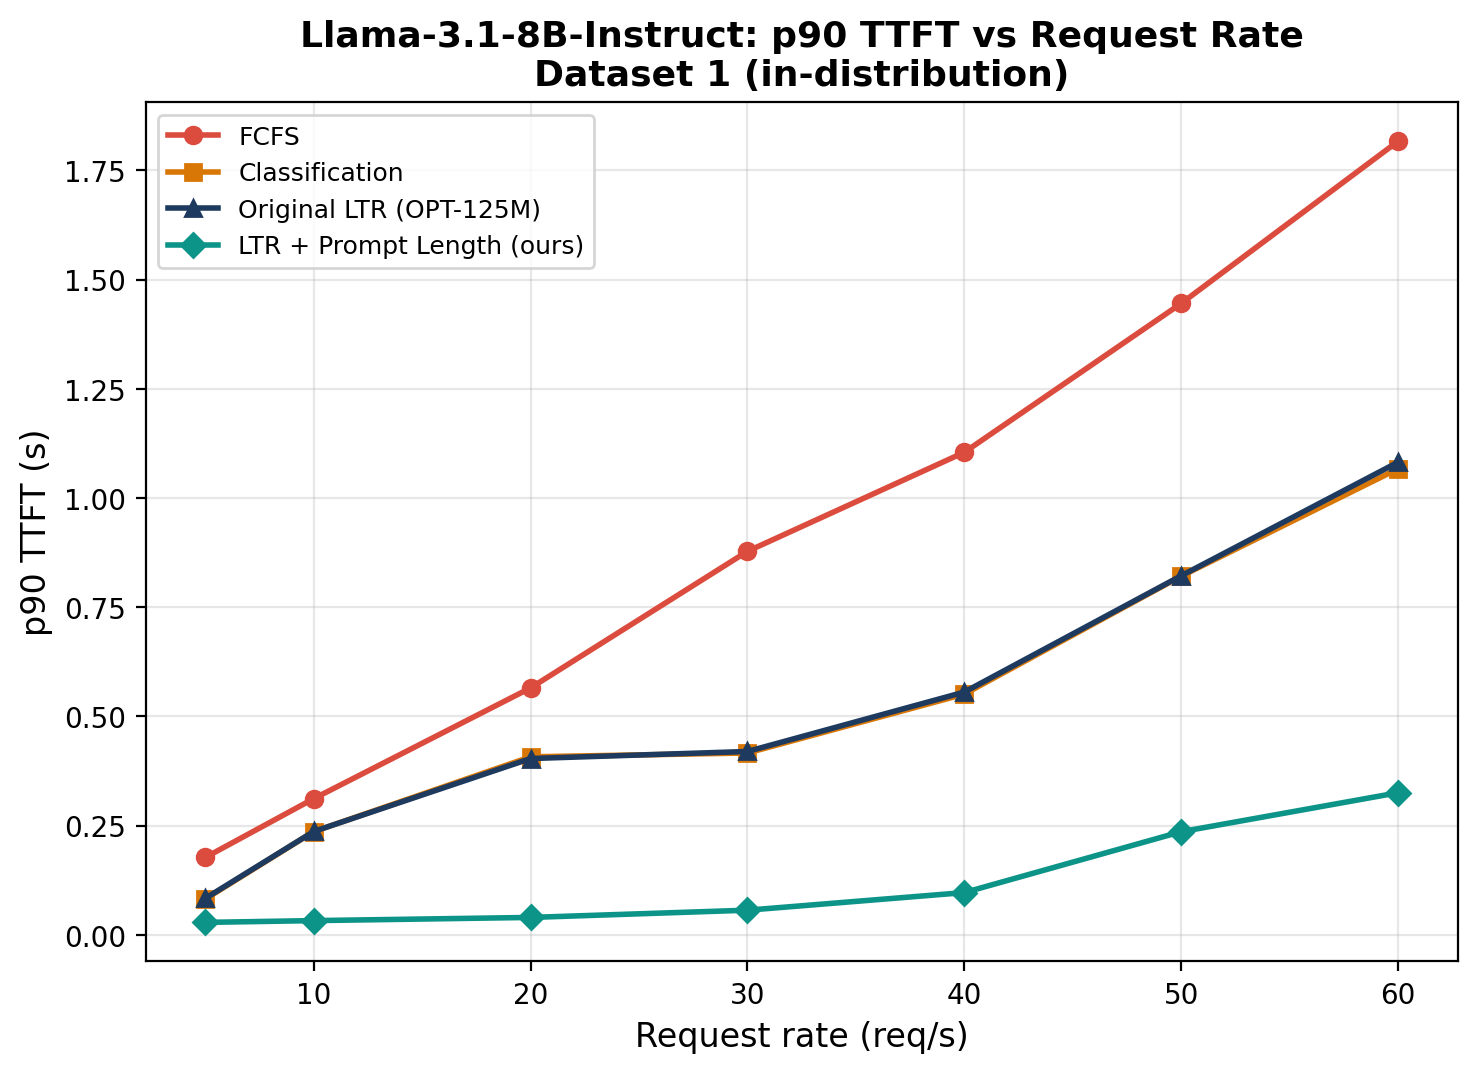
\includegraphics[width=\linewidth]{figures/ttft_p90_dataset1.png}
        \caption{Dataset 1 (in-distribution)}
        \label{fig:ttft-d1}
    \end{subfigure}
    \hfill
    \begin{subfigure}[b]{0.48\textwidth}
        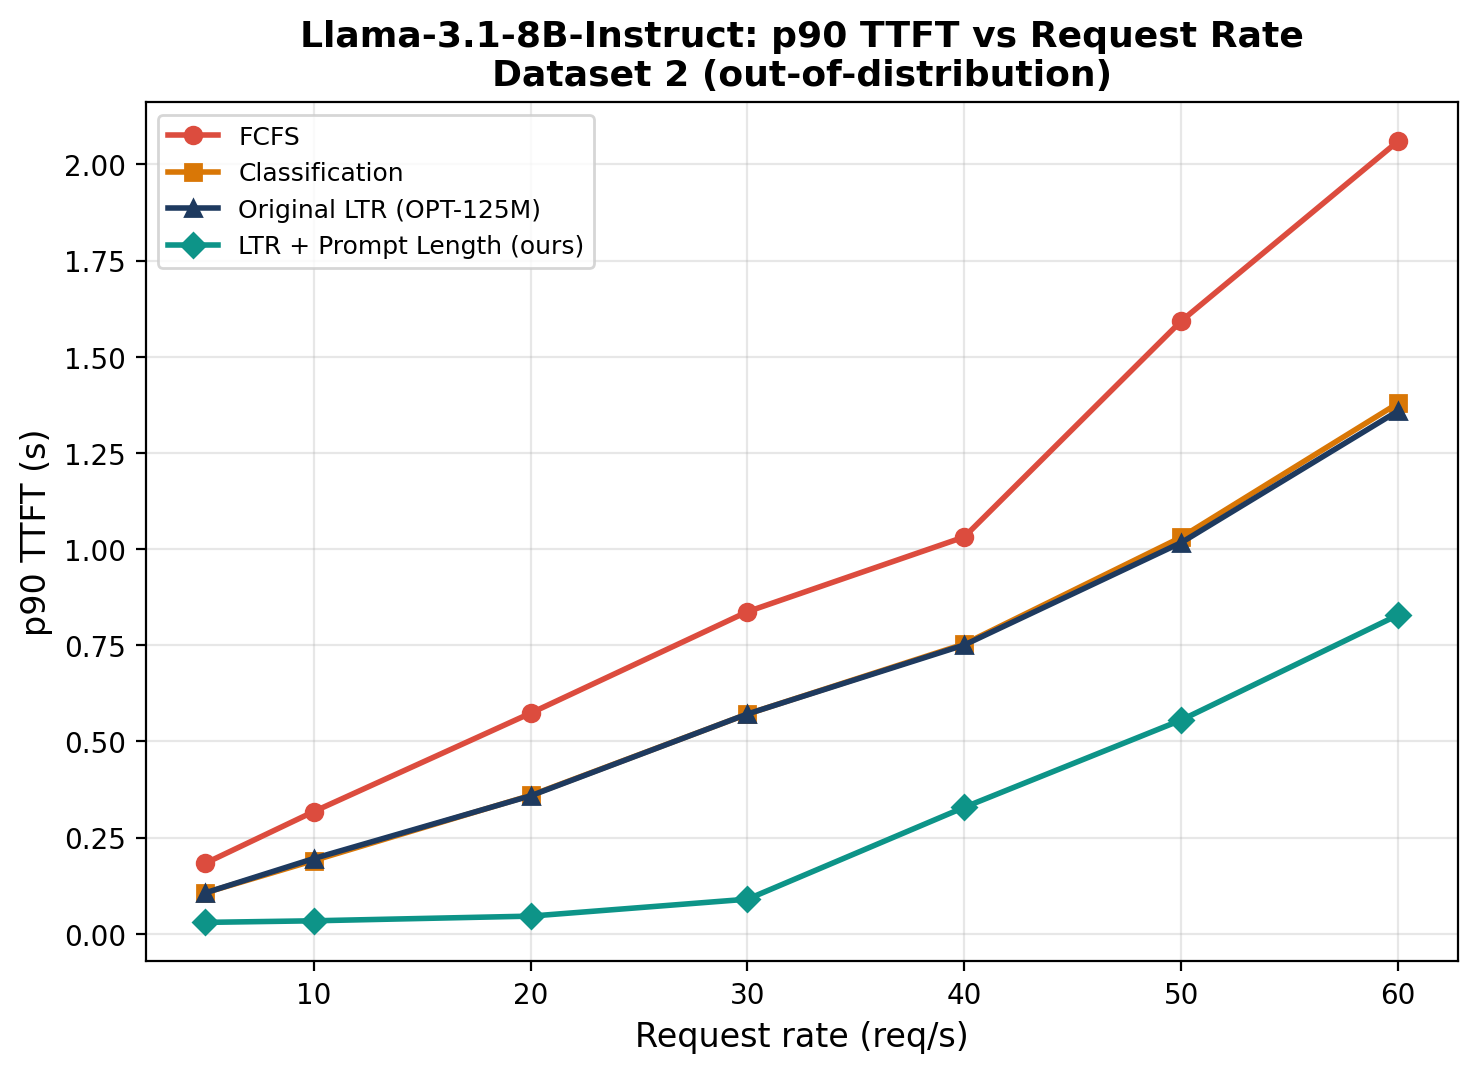
\includegraphics[width=\linewidth]{figures/ttft_p90_dataset2.png}
        \caption{Dataset 2 (out-of-distribution)}
        \label{fig:ttft-d2}
    \end{subfigure}
    \begin{subfigure}[b]{0.48\textwidth}
        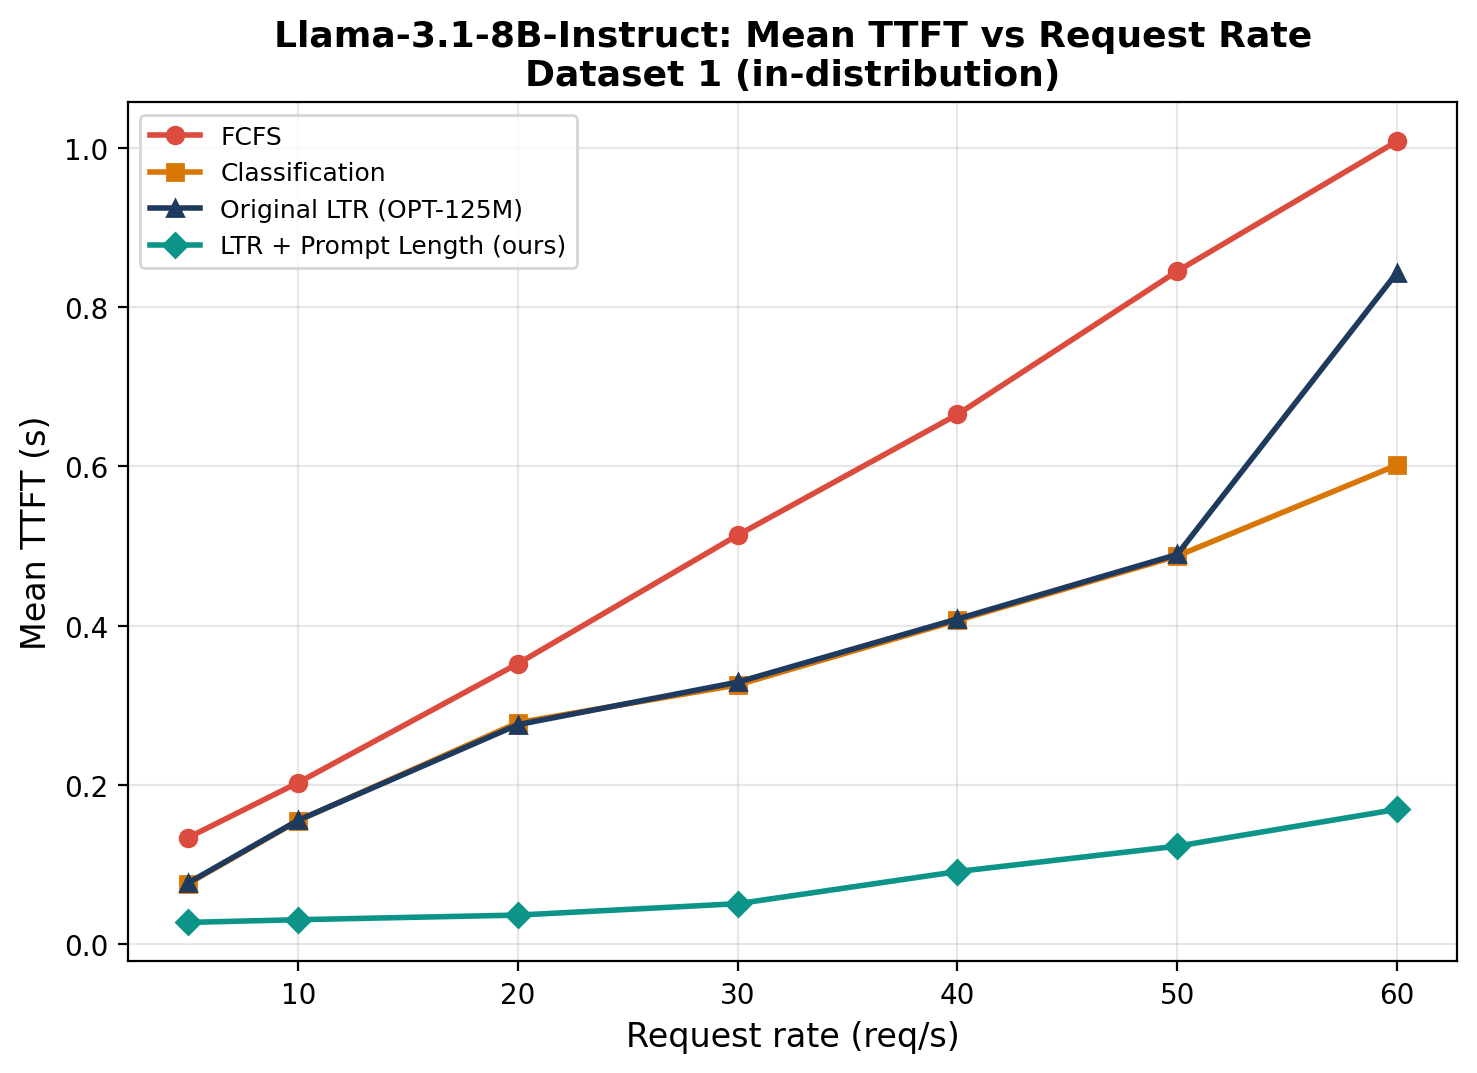
\includegraphics[width=\linewidth]{figures/ttft_mean_dataset1.png}
        \caption{Dataset 1 (in-distribution)}
        \label{fig:ttft-d1}
    \end{subfigure}
    \hfill
    \begin{subfigure}[b]{0.48\textwidth}
        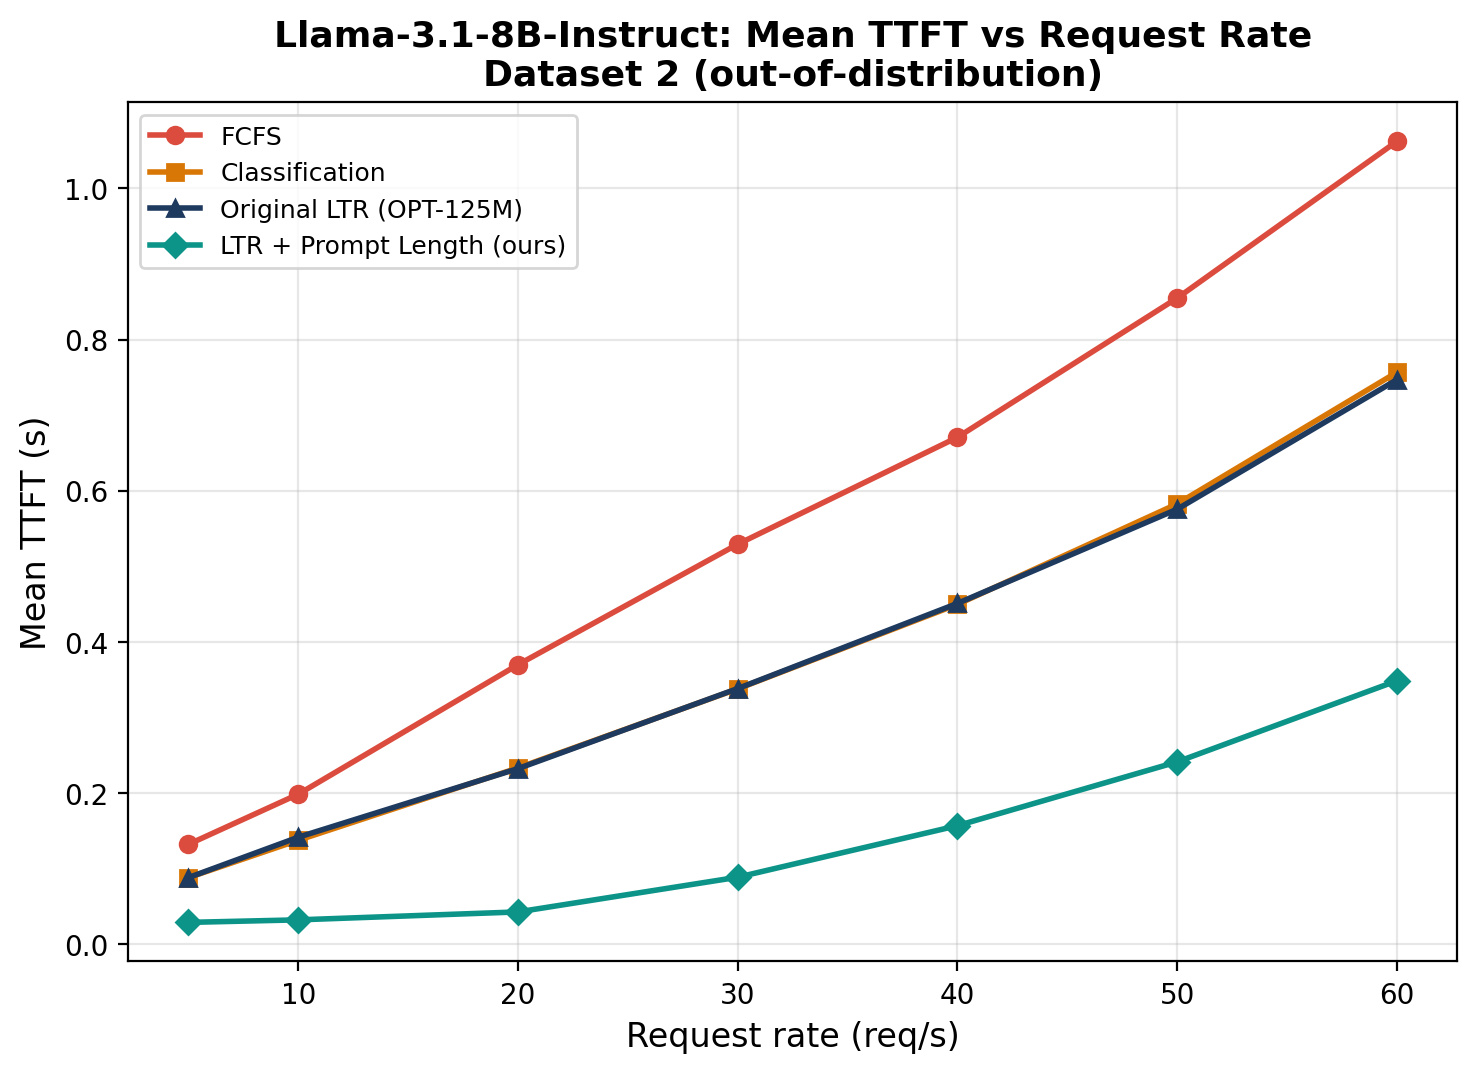
\includegraphics[width=\linewidth]{figures/ttft_mean_dataset2.png}
        \caption{Dataset 2 (out-of-distribution)}
        \label{fig:ttft-d2}
    \end{subfigure}
    \caption{Mean and p90 time-to-first-token versus request rate, by
    scheduler.}
    \label{fig:ttft-vs-rate}
\end{figure*}

\input{tables/hol_blocking}
\input{tables/hol_blocking}
\input{tables/gpu_utilization}
\input{tables/kendalls_tau}

\subsection{Head-of-Line Blocking Indicators}
\label{subsec:results-hol}

Table~\ref{tab:hol_blocking} and Figure~\ref{fig:hol-blocking} summarize the
p90/mean latency ratio at high load and the latency-vs-rate slope for each
scheduler. The Classification and original LTR schedulers achieve the lowest
p90/mean ratio on Dataset~1, indicating that when their length estimate is
accurate, they compress tail latency effectively; however, both show a
steeper latency-vs-rate slope than FCFS on Dataset~1, meaning their latency
degrades faster as load increases. LTR + Prompt Length achieves the lowest
latency-vs-rate slope on Dataset~2 (the out-of-distribution set) among all
four policies, consistent with the intuition that the prompt-length signal
provides a stabilizing effect precisely when the learned predictor is
operating outside its training distribution. Notably, LTR + Prompt Length's p90/mean ratio on Dataset 2 is nonetheless the highest of the four schedulers, indicating that its tail latency still grows in proportion to its mean under distribution shift even as that growth compounds more slowly across increasing request rates than it does for the other three policies. FCFS's slope on Dataset 1 is the flattest of the four despite its poor tail-latency ratio, underscoring that these two indicators capture distinct aspects of HOL blocking rather than a single underlying quantity.

\begin{figure}[H]
    \centering

    \begin{subfigure}{\linewidth}
        \centering
        \includegraphics[width=\linewidth]{figures/hol_blocking_ratio.png}
        \caption{p90/mean latency ratio at high load}
        \label{fig:hol-ratio}
    \end{subfigure}

    \vspace{2mm}

    \begin{subfigure}{\linewidth}
        \centering
        \includegraphics[width=\linewidth]{figures/hol_blocking_slope.png}
        \caption{Latency-vs-request-rate slope}
        \label{fig:hol-slope}
    \end{subfigure}

    \caption{HOL blocking indicators by scheduler and dataset.}
    \label{fig:hol-blocking}
\end{figure}
\subsection{GPU Resource Utilization}
\label{subsec:results-gpu}

Table~\ref{tab:gpu_utilization} and Figure~\ref{fig:gpu-utilization} report
peak GPU memory allocation and utilization measured while serving each
dataset. Memory utilization remains above 86\% of the profiled budget on both
datasets, indicating that the composite scheduler's reordering step does not
introduce additional memory overhead relative to the serving engine's
baseline footprint; the reordering computation itself operates on tokenized
prompt lengths and predictor scores, both of which are negligible in memory
compared to the model weights and KV cache.



\subsection{Ranking Quality: Kendall's Tau}
\label{subsec:results-tau}

Table~\ref{tab:kendalls_tau} reports Kendall's tau between each score and the
true output length on the Dataset~2 (out-of-distribution) held-out set. The
composite score achieves a small improvement over the LTR-only score
(0.3445 to 0.3457, $\Delta = +0.0011$), indicating that the prompt-length
signal does not degrade ranking quality under distribution shift and offers a
modest, consistent improvement even independent of its effect on the
scheduling-level metrics reported above.
\begin{figure}[H]
    \centering
    \includegraphics[width=0.85\linewidth,height=5.2cm,keepaspectratio]{figures/gpu_utilization.png}
    \caption{Peak GPU memory allocation, peak reserved memory, and memory
    utilization by dataset.}
    \label{fig:gpu-utilization}
\end{figure}
\subsection{Throughput by Scheduler, Averaged Across Request Rates}
\label{subsec:results-throughput-avg}

Figure~\ref{fig:throughput-avg} presents the same throughput comparison as
Table~\ref{tab:throughput} averaged across all seven tested request rates
rather than aggregated once per dataset, confirming that the ordering in
Table~\ref{tab:throughput} is not an artifact of any single request rate.

\begin{figure}[H]
    \centering
    \includegraphics[width=0.85\linewidth,height=5.0cm,keepaspectratio]{figures/throughput_by_scheduler.png}
    \caption{Mean throughput by scheduler, averaged across all tested
    request rates.}
    \label{fig:throughput-avg}
\end{figure}

\FloatBarrier
\input{sections/discussion}
\FloatBarrier
\input{sections/conclusion}
\FloatBarrier
\appendices 
\section{} 
\label{sec:appendix} 
\vspace{1em}
\begin{center} 
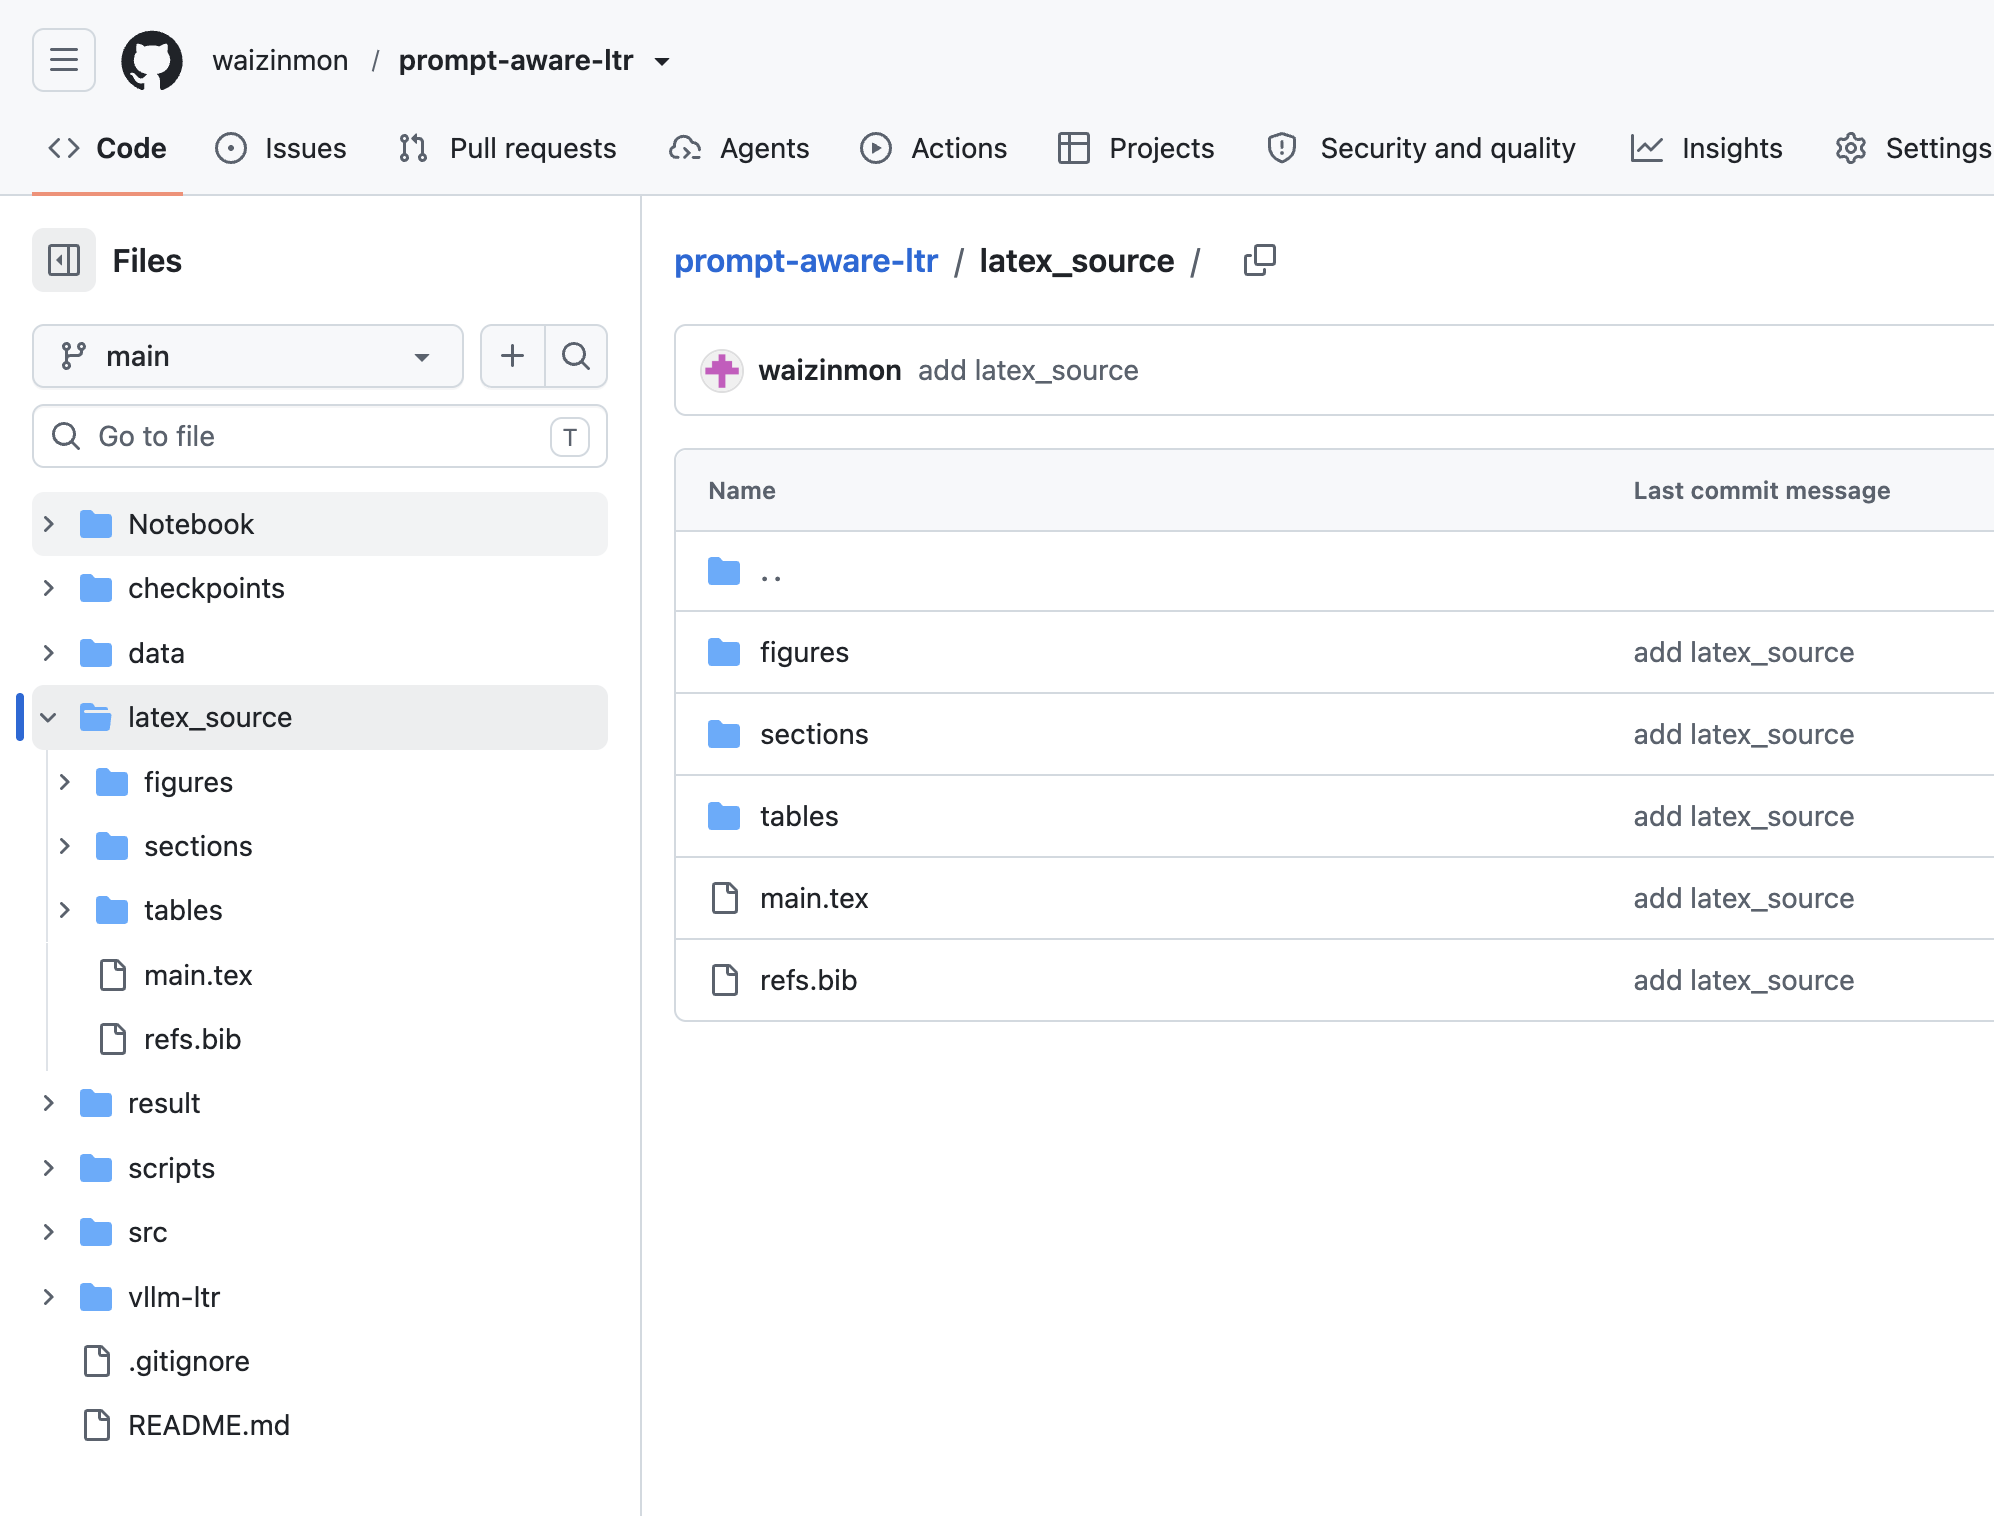
\includegraphics[width=0.85\linewidth]{figures/appendix_latex_source_screenshot.png} 
\end{center} 

\label{sec:references}
\bibliographystyle{IEEEtran}
\bibliography{refs}

\end{document}
